%\documentclass[pra,showpacs,showkeys,amsfonts,amsmath,twocolumn,handou]{revtex4}
\documentclass[amsmath,blue,table,sans,handout]{beamer}
%\documentclass[pra,showpacs,showkeys,amsfonts]{revtex4}
\usepackage[T1]{fontenc}
%%\usepackage{beamerthemeshadow}
\usepackage[headheight=1pt,footheight=10pt]{beamerthemeboxes}
\addfootboxtemplate{\color{structure!80}}{\color{white}\tiny \hfill Karl Svozil (TU Vienna)\hfill}
\addfootboxtemplate{\color{structure!65}}{\color{white}\tiny \hfill Q \& Quasi-Classical Correlations $\ldots$\hfill}
\addfootboxtemplate{\color{structure!50}}{\color{white}\tiny \hfill Bratislava, March  6th, 2008\hfill}
%\usepackage[dark]{beamerthemesidebar}
%\usepackage[headheight=24pt,footheight=12pt]{beamerthemesplit}
%\usepackage{beamerthemesplit}
%\usepackage[bar]{beamerthemetree}
\usepackage{graphicx}
\usepackage{pgf}
%\usepackage[usenames]{color}
%\newcommand{\Red}{\color{Red}}  %(VERY-Approx.PANTONE-RED)
%\newcommand{\Green}{\color{Green}}  %(VERY-Approx.PANTONE-GREEN)

%\RequirePackage[german]{babel}
%\selectlanguage{german}
%\RequirePackage[isolatin]{inputenc}

\pgfdeclareimage[height=0.5cm]{logo}{tu-logo}
\logo{\pgfuseimage{logo}}
\beamertemplatetriangleitem
%\beamertemplateballitem

\beamerboxesdeclarecolorscheme{alert}{red}{red!15!averagebackgroundcolor}
%\begin{beamerboxesrounded}[scheme=alert,shadow=true]{}
%\end{beamerboxesrounded}

%\beamersetaveragebackground{green!10}

%\beamertemplatecircleminiframe

\begin{document}

\title{\bf \textcolor{blue}{Quantum and Quasi-Classical Correlations \& the Cost of Breaking the Bell Barrier}}
%\subtitle{Naturwissenschaftlich-Humanisticher Tag am BG 19\\Weltbild und Wissenschaft\\http://tph.tuwien.ac.at/\~{}svozil/publ/2005-BG18-pres.pdf}
\subtitle{\textcolor{orange!60}{\small http://tph.tuwien.ac.at/$\sim$svozil/publ/2008-bratislava-pres.pdf}}
\author{Karl Svozil}
\institute{Institut f\"ur Theoretische Physik, University of Technology Vienna, \\
Wiedner Hauptstra\ss e 8-10/136, A-1040 Vienna, Austria\\
svozil@tuwien.ac.at
%{\tiny Disclaimer: Die hier vertretenen Meinungen des Autors verstehen sich als Diskussionsbeitr�ge und decken sich nicht notwendigerweise mit den Positionen der Technischen Universit�t Wien oder deren Vertreter.}
}
\date{Bratislava, Slovak Republic, March  6th, 2008}
\maketitle



\frame{
\frametitle{Contents}
\tableofcontents
}



\section{Classical, quantum \& stronger-than-quantum correlations}

\frame{
\frametitle{Main results}

\begin{itemize}
\item<1->
Classical protocol with a single bit exchange renders a
correlation function with a maximal violation of the
Clauser-Horne-Shimony-Holt inequality of 4.

\item<1->
Computation of exact quantum bounds for Bell-type inequalities.
\end{itemize}

}

\subsection{General setup for two-particle correlations}
\frame{
\frametitle{General setup for two-particle correlations}

\begin{itemize}
\item<1->
Two measurement directions ${ a}$ \& ${ b}$
of two
dichotomic observables
$O({ a})$ \&
$O({ b})$
with values ``-1'' or ``1''
at two spatially separated locations.
\item<1->
The measurement direction ${a}$ at ``Alice's location''
is unknown to an observer ``Bob'' measuring ${ b}$ and {\it vice versa}.
\item<1->
A two-particle correlation function $E(a,b )$
is defined by averaging over the product of the outcomes $O({ a})_i, O({ b} )_i\in \{-1,1\}$
in the $i$th experiment for a total of $N$ experiments; i.e.,  $$E(a,b )={1\over N}\sum_{i=1}^N O({ a})_i O({ b})_i$$
\end{itemize}
}


\subsection{Classical correlations}

\frame{
\frametitle{Classical correlations for two-particle ``perfect correlation''}
Assume uniform  distribution of (opposite) ``angular momenta''
of the two particles; Alice measuring along angle $a$, Bob measuring along $b$:

\begin{center}
%TexCad Options
%\grade{\on}
%\emlines{\off}
%\beziermacro{\on}
%\reduce{\on}
%\snapping{\off}
%\quality{8.00}
%\graddiff{0.01}
%\snapasp{1}
%\zoom{0.60}
\unitlength 0.40mm
\linethickness{0.4pt}
\begin{picture}(220.35,68.50)
(0,0)
%\circle(30.25,29.75){61.53}
\put(30.25,60.52){\line(1,0){1.23}}
\put(31.48,60.49){\line(1,0){1.22}}
\multiput(32.70,60.42)(0.61,-0.06){2}{\line(1,0){0.61}}
\multiput(33.92,60.30)(0.61,-0.09){2}{\line(1,0){0.61}}
\multiput(35.14,60.12)(0.60,-0.11){2}{\line(1,0){0.60}}
\multiput(36.34,59.91)(0.40,-0.09){3}{\line(1,0){0.40}}
\multiput(37.54,59.64)(0.40,-0.10){3}{\line(1,0){0.40}}
\multiput(38.73,59.32)(0.29,-0.09){4}{\line(1,0){0.29}}
\multiput(39.90,58.96)(0.29,-0.10){4}{\line(1,0){0.29}}
\multiput(41.06,58.55)(0.28,-0.11){4}{\line(1,0){0.28}}
\multiput(42.20,58.10)(0.22,-0.10){5}{\line(1,0){0.22}}
\multiput(43.32,57.60)(0.22,-0.11){5}{\line(1,0){0.22}}
\multiput(44.42,57.06)(0.22,-0.12){5}{\line(1,0){0.22}}
\multiput(45.50,56.47)(0.18,-0.10){6}{\line(1,0){0.18}}
\multiput(46.55,55.84)(0.17,-0.11){6}{\line(1,0){0.17}}
\multiput(47.58,55.17)(0.17,-0.12){6}{\line(1,0){0.17}}
\multiput(48.58,54.46)(0.14,-0.11){7}{\line(1,0){0.14}}
\multiput(49.55,53.71)(0.13,-0.11){7}{\line(1,0){0.13}}
\multiput(50.49,52.92)(0.13,-0.12){7}{\line(1,0){0.13}}
\multiput(51.40,52.10)(0.11,-0.11){8}{\line(1,0){0.11}}
\multiput(52.27,51.23)(0.12,-0.13){7}{\line(0,-1){0.13}}
\multiput(53.11,50.34)(0.11,-0.13){7}{\line(0,-1){0.13}}
\multiput(53.91,49.41)(0.11,-0.14){7}{\line(0,-1){0.14}}
\multiput(54.68,48.45)(0.10,-0.14){7}{\line(0,-1){0.14}}
\multiput(55.40,47.46)(0.11,-0.17){6}{\line(0,-1){0.17}}
\multiput(56.09,46.45)(0.11,-0.17){6}{\line(0,-1){0.17}}
\multiput(56.74,45.40)(0.10,-0.18){6}{\line(0,-1){0.18}}
\multiput(57.34,44.33)(0.11,-0.22){5}{\line(0,-1){0.22}}
\multiput(57.90,43.24)(0.10,-0.22){5}{\line(0,-1){0.22}}
\multiput(58.41,42.13)(0.12,-0.28){4}{\line(0,-1){0.28}}
\multiput(58.89,41.00)(0.11,-0.29){4}{\line(0,-1){0.29}}
\multiput(59.31,39.85)(0.09,-0.29){4}{\line(0,-1){0.29}}
\multiput(59.69,38.68)(0.11,-0.39){3}{\line(0,-1){0.39}}
\multiput(60.02,37.50)(0.10,-0.40){3}{\line(0,-1){0.40}}
\multiput(60.31,36.30)(0.12,-0.60){2}{\line(0,-1){0.60}}
\multiput(60.55,35.10)(0.09,-0.61){2}{\line(0,-1){0.61}}
\multiput(60.74,33.89)(0.07,-0.61){2}{\line(0,-1){0.61}}
\put(60.88,32.67){\line(0,-1){1.22}}
\put(60.97,31.45){\line(0,-1){1.23}}
\put(61.01,30.22){\line(0,-1){1.23}}
\put(61.01,28.99){\line(0,-1){1.23}}
\put(60.95,27.77){\line(0,-1){1.22}}
\multiput(60.85,26.54)(-0.08,-0.61){2}{\line(0,-1){0.61}}
\multiput(60.70,25.33)(-0.10,-0.61){2}{\line(0,-1){0.61}}
\multiput(60.49,24.12)(-0.08,-0.40){3}{\line(0,-1){0.40}}
\multiput(60.25,22.91)(-0.10,-0.40){3}{\line(0,-1){0.40}}
\multiput(59.95,21.72)(-0.11,-0.39){3}{\line(0,-1){0.39}}
\multiput(59.61,20.55)(-0.10,-0.29){4}{\line(0,-1){0.29}}
\multiput(59.22,19.38)(-0.11,-0.29){4}{\line(0,-1){0.29}}
\multiput(58.78,18.24)(-0.10,-0.23){5}{\line(0,-1){0.23}}
\multiput(58.30,17.11)(-0.11,-0.22){5}{\line(0,-1){0.22}}
\multiput(57.77,16.00)(-0.11,-0.22){5}{\line(0,-1){0.22}}
\multiput(57.20,14.91)(-0.10,-0.18){6}{\line(0,-1){0.18}}
\multiput(56.59,13.85)(-0.11,-0.17){6}{\line(0,-1){0.17}}
\multiput(55.93,12.81)(-0.12,-0.17){6}{\line(0,-1){0.17}}
\multiput(55.24,11.80)(-0.11,-0.14){7}{\line(0,-1){0.14}}
\multiput(54.50,10.82)(-0.11,-0.14){7}{\line(0,-1){0.14}}
\multiput(53.73,9.87)(-0.12,-0.13){7}{\line(0,-1){0.13}}
\multiput(52.92,8.95)(-0.11,-0.11){8}{\line(0,-1){0.11}}
\multiput(52.07,8.06)(-0.11,-0.11){8}{\line(-1,0){0.11}}
\multiput(51.19,7.21)(-0.13,-0.12){7}{\line(-1,0){0.13}}
\multiput(50.27,6.39)(-0.14,-0.11){7}{\line(-1,0){0.14}}
\multiput(49.32,5.61)(-0.14,-0.11){7}{\line(-1,0){0.14}}
\multiput(48.35,4.87)(-0.17,-0.12){6}{\line(-1,0){0.17}}
\multiput(47.34,4.17)(-0.17,-0.11){6}{\line(-1,0){0.17}}
\multiput(46.30,3.51)(-0.18,-0.10){6}{\line(-1,0){0.18}}
\multiput(45.25,2.89)(-0.22,-0.12){5}{\line(-1,0){0.22}}
\multiput(44.16,2.31)(-0.22,-0.11){5}{\line(-1,0){0.22}}
\multiput(43.06,1.78)(-0.23,-0.10){5}{\line(-1,0){0.23}}
\multiput(41.93,1.29)(-0.29,-0.11){4}{\line(-1,0){0.29}}
\multiput(40.79,0.85)(-0.29,-0.10){4}{\line(-1,0){0.29}}
\multiput(39.63,0.45)(-0.39,-0.12){3}{\line(-1,0){0.39}}
\multiput(38.45,0.10)(-0.40,-0.10){3}{\line(-1,0){0.40}}
\multiput(37.26,-0.21)(-0.40,-0.09){3}{\line(-1,0){0.40}}
\multiput(36.06,-0.46)(-0.60,-0.10){2}{\line(-1,0){0.60}}
\multiput(34.85,-0.67)(-0.61,-0.08){2}{\line(-1,0){0.61}}
\put(33.64,-0.83){\line(-1,0){1.22}}
\put(32.41,-0.94){\line(-1,0){1.23}}
\put(31.19,-1.00){\line(-1,0){1.23}}
\put(29.96,-1.01){\line(-1,0){1.23}}
\put(28.74,-0.98){\line(-1,0){1.22}}
\multiput(27.51,-0.89)(-0.61,0.07){2}{\line(-1,0){0.61}}
\multiput(26.29,-0.76)(-0.61,0.09){2}{\line(-1,0){0.61}}
\multiput(25.08,-0.58)(-0.60,0.12){2}{\line(-1,0){0.60}}
\multiput(23.87,-0.35)(-0.40,0.09){3}{\line(-1,0){0.40}}
\multiput(22.68,-0.07)(-0.39,0.11){3}{\line(-1,0){0.39}}
\multiput(21.49,0.26)(-0.29,0.09){4}{\line(-1,0){0.29}}
\multiput(20.33,0.63)(-0.29,0.10){4}{\line(-1,0){0.29}}
\multiput(19.17,1.05)(-0.28,0.12){4}{\line(-1,0){0.28}}
\multiput(18.04,1.51)(-0.22,0.10){5}{\line(-1,0){0.22}}
\multiput(16.92,2.02)(-0.22,0.11){5}{\line(-1,0){0.22}}
\multiput(15.83,2.58)(-0.21,0.12){5}{\line(-1,0){0.21}}
\multiput(14.75,3.17)(-0.17,0.11){6}{\line(-1,0){0.17}}
\multiput(13.71,3.81)(-0.17,0.11){6}{\line(-1,0){0.17}}
\multiput(12.68,4.49)(-0.14,0.10){7}{\line(-1,0){0.14}}
\multiput(11.69,5.21)(-0.14,0.11){7}{\line(-1,0){0.14}}
\multiput(10.73,5.97)(-0.13,0.11){7}{\line(-1,0){0.13}}
\multiput(9.80,6.77)(-0.13,0.12){7}{\line(-1,0){0.13}}
\multiput(8.90,7.60)(-0.11,0.11){8}{\line(0,1){0.11}}
\multiput(8.03,8.47)(-0.12,0.13){7}{\line(0,1){0.13}}
\multiput(7.20,9.38)(-0.11,0.13){7}{\line(0,1){0.13}}
\multiput(6.40,10.31)(-0.11,0.14){7}{\line(0,1){0.14}}
\multiput(5.65,11.28)(-0.12,0.17){6}{\line(0,1){0.17}}
\multiput(4.93,12.27)(-0.11,0.17){6}{\line(0,1){0.17}}
\multiput(4.25,13.30)(-0.11,0.17){6}{\line(0,1){0.17}}
\multiput(3.62,14.35)(-0.12,0.21){5}{\line(0,1){0.21}}
\multiput(3.03,15.42)(-0.11,0.22){5}{\line(0,1){0.22}}
\multiput(2.48,16.52)(-0.10,0.22){5}{\line(0,1){0.22}}
\multiput(1.97,17.64)(-0.12,0.28){4}{\line(0,1){0.28}}
\multiput(1.51,18.77)(-0.10,0.29){4}{\line(0,1){0.29}}
\multiput(1.10,19.93)(-0.09,0.29){4}{\line(0,1){0.29}}
\multiput(0.73,21.10)(-0.11,0.39){3}{\line(0,1){0.39}}
\multiput(0.41,22.28)(-0.09,0.40){3}{\line(0,1){0.40}}
\multiput(0.13,23.48)(-0.11,0.60){2}{\line(0,1){0.60}}
\multiput(-0.10,24.68)(-0.09,0.61){2}{\line(0,1){0.61}}
\multiput(-0.27,25.90)(-0.06,0.61){2}{\line(0,1){0.61}}
\put(-0.40,27.12){\line(0,1){1.22}}
\put(-0.48,28.34){\line(0,1){1.23}}
\put(-0.51,29.57){\line(0,1){1.23}}
\put(-0.50,30.80){\line(0,1){1.23}}
\put(-0.43,32.02){\line(0,1){1.22}}
\multiput(-0.32,33.24)(0.08,0.61){2}{\line(0,1){0.61}}
\multiput(-0.15,34.46)(0.11,0.60){2}{\line(0,1){0.60}}
\multiput(0.06,35.67)(0.09,0.40){3}{\line(0,1){0.40}}
\multiput(0.32,36.87)(0.10,0.40){3}{\line(0,1){0.40}}
\multiput(0.63,38.05)(0.12,0.39){3}{\line(0,1){0.39}}
\multiput(0.98,39.23)(0.10,0.29){4}{\line(0,1){0.29}}
\multiput(1.38,40.39)(0.11,0.29){4}{\line(0,1){0.29}}
\multiput(1.83,41.53)(0.10,0.22){5}{\line(0,1){0.22}}
\multiput(2.32,42.65)(0.11,0.22){5}{\line(0,1){0.22}}
\multiput(2.86,43.76)(0.12,0.22){5}{\line(0,1){0.22}}
\multiput(3.44,44.84)(0.10,0.18){6}{\line(0,1){0.18}}
\multiput(4.06,45.90)(0.11,0.17){6}{\line(0,1){0.17}}
\multiput(4.73,46.93)(0.12,0.17){6}{\line(0,1){0.17}}
\multiput(5.43,47.93)(0.11,0.14){7}{\line(0,1){0.14}}
\multiput(6.18,48.91)(0.11,0.13){7}{\line(0,1){0.13}}
\multiput(6.96,49.85)(0.12,0.13){7}{\line(0,1){0.13}}
\multiput(7.78,50.76)(0.11,0.11){8}{\line(0,1){0.11}}
\multiput(8.64,51.64)(0.11,0.11){8}{\line(1,0){0.11}}
\multiput(9.53,52.49)(0.13,0.12){7}{\line(1,0){0.13}}
\multiput(10.45,53.30)(0.14,0.11){7}{\line(1,0){0.14}}
\multiput(11.40,54.07)(0.14,0.10){7}{\line(1,0){0.14}}
\multiput(12.39,54.80)(0.17,0.12){6}{\line(1,0){0.17}}
\multiput(13.40,55.49)(0.17,0.11){6}{\line(1,0){0.17}}
\multiput(14.44,56.14)(0.18,0.10){6}{\line(1,0){0.18}}
\multiput(15.51,56.75)(0.22,0.11){5}{\line(1,0){0.22}}
\multiput(16.60,57.32)(0.22,0.10){5}{\line(1,0){0.22}}
\multiput(17.71,57.84)(0.28,0.12){4}{\line(1,0){0.28}}
\multiput(18.84,58.32)(0.29,0.11){4}{\line(1,0){0.29}}
\multiput(19.98,58.75)(0.29,0.10){4}{\line(1,0){0.29}}
\multiput(21.15,59.14)(0.39,0.11){3}{\line(1,0){0.39}}
\multiput(22.33,59.48)(0.40,0.10){3}{\line(1,0){0.40}}
\multiput(23.52,59.77)(0.40,0.08){3}{\line(1,0){0.40}}
\multiput(24.72,60.01)(0.61,0.10){2}{\line(1,0){0.61}}
\multiput(25.93,60.21)(0.61,0.07){2}{\line(1,0){0.61}}
\put(27.15,60.36){\line(1,0){1.22}}
\put(28.37,60.46){\line(1,0){1.88}}
%\end
\put(30.25,30.25){\line(0,1){30.50}}
%\dottedline(1.75,235.75)(2,235.25)
\multiput(1.68,235.68)(.125,-.25){3}{{\rule{.4pt}{.4pt}}}
\put(0.00,0.00){}
%\dottedline(2,235.25)(63.5,234.75)
\multiput(1.93,235.18)(.99194,-.00806){63}{{\rule{.4pt}{.4pt}}}
\put(0.00,0.00){}
%\dottedline(9.5,255.5)(55.75,214.25)
\multiput(9.43,255.43)(.72266,-.64453){65}{{\rule{.4pt}{.4pt}}}
\put(0.00,0.00){}
\put(30.25,68.50){\makebox(0,0)[cc]{$a$}}
%\emline(0.00,30.00)(61.00,30.00)
\put(0.00,30.00){\line(1,0){61.00}}
%\end
%\circle(109.92,29.75){61.53}
\put(109.92,60.52){\line(1,0){1.23}}
\put(111.15,60.49){\line(1,0){1.22}}
\multiput(112.37,60.42)(0.61,-0.06){2}{\line(1,0){0.61}}
\multiput(113.59,60.30)(0.61,-0.09){2}{\line(1,0){0.61}}
\multiput(114.81,60.12)(0.60,-0.11){2}{\line(1,0){0.60}}
\multiput(116.01,59.91)(0.40,-0.09){3}{\line(1,0){0.40}}
\multiput(117.21,59.64)(0.40,-0.10){3}{\line(1,0){0.40}}
\multiput(118.40,59.32)(0.29,-0.09){4}{\line(1,0){0.29}}
\multiput(119.57,58.96)(0.29,-0.10){4}{\line(1,0){0.29}}
\multiput(120.73,58.55)(0.28,-0.11){4}{\line(1,0){0.28}}
\multiput(121.87,58.10)(0.22,-0.10){5}{\line(1,0){0.22}}
\multiput(122.99,57.60)(0.22,-0.11){5}{\line(1,0){0.22}}
\multiput(124.09,57.06)(0.22,-0.12){5}{\line(1,0){0.22}}
\multiput(125.17,56.47)(0.18,-0.10){6}{\line(1,0){0.18}}
\multiput(126.22,55.84)(0.17,-0.11){6}{\line(1,0){0.17}}
\multiput(127.25,55.17)(0.17,-0.12){6}{\line(1,0){0.17}}
\multiput(128.25,54.46)(0.14,-0.11){7}{\line(1,0){0.14}}
\multiput(129.22,53.71)(0.13,-0.11){7}{\line(1,0){0.13}}
\multiput(130.16,52.92)(0.13,-0.12){7}{\line(1,0){0.13}}
\multiput(131.07,52.10)(0.11,-0.11){8}{\line(1,0){0.11}}
\multiput(131.94,51.23)(0.12,-0.13){7}{\line(0,-1){0.13}}
\multiput(132.78,50.34)(0.11,-0.13){7}{\line(0,-1){0.13}}
\multiput(133.58,49.41)(0.11,-0.14){7}{\line(0,-1){0.14}}
\multiput(134.35,48.45)(0.10,-0.14){7}{\line(0,-1){0.14}}
\multiput(135.07,47.46)(0.11,-0.17){6}{\line(0,-1){0.17}}
\multiput(135.76,46.45)(0.11,-0.17){6}{\line(0,-1){0.17}}
\multiput(136.41,45.40)(0.10,-0.18){6}{\line(0,-1){0.18}}
\multiput(137.01,44.33)(0.11,-0.22){5}{\line(0,-1){0.22}}
\multiput(137.57,43.24)(0.10,-0.22){5}{\line(0,-1){0.22}}
\multiput(138.08,42.13)(0.12,-0.28){4}{\line(0,-1){0.28}}
\multiput(138.56,41.00)(0.11,-0.29){4}{\line(0,-1){0.29}}
\multiput(138.98,39.85)(0.09,-0.29){4}{\line(0,-1){0.29}}
\multiput(139.36,38.68)(0.11,-0.39){3}{\line(0,-1){0.39}}
\multiput(139.69,37.50)(0.10,-0.40){3}{\line(0,-1){0.40}}
\multiput(139.98,36.30)(0.12,-0.60){2}{\line(0,-1){0.60}}
\multiput(140.22,35.10)(0.09,-0.61){2}{\line(0,-1){0.61}}
\multiput(140.41,33.89)(0.07,-0.61){2}{\line(0,-1){0.61}}
\put(140.55,32.67){\line(0,-1){1.22}}
\put(140.64,31.45){\line(0,-1){1.23}}
\put(140.68,30.22){\line(0,-1){1.23}}
\put(140.68,28.99){\line(0,-1){1.23}}
\put(140.62,27.77){\line(0,-1){1.22}}
\multiput(140.52,26.54)(-0.08,-0.61){2}{\line(0,-1){0.61}}
\multiput(140.37,25.33)(-0.10,-0.61){2}{\line(0,-1){0.61}}
\multiput(140.16,24.12)(-0.08,-0.40){3}{\line(0,-1){0.40}}
\multiput(139.92,22.91)(-0.10,-0.40){3}{\line(0,-1){0.40}}
\multiput(139.62,21.72)(-0.11,-0.39){3}{\line(0,-1){0.39}}
\multiput(139.28,20.55)(-0.10,-0.29){4}{\line(0,-1){0.29}}
\multiput(138.89,19.38)(-0.11,-0.29){4}{\line(0,-1){0.29}}
\multiput(138.45,18.24)(-0.10,-0.23){5}{\line(0,-1){0.23}}
\multiput(137.97,17.11)(-0.11,-0.22){5}{\line(0,-1){0.22}}
\multiput(137.44,16.00)(-0.11,-0.22){5}{\line(0,-1){0.22}}
\multiput(136.87,14.91)(-0.10,-0.18){6}{\line(0,-1){0.18}}
\multiput(136.26,13.85)(-0.11,-0.17){6}{\line(0,-1){0.17}}
\multiput(135.60,12.81)(-0.12,-0.17){6}{\line(0,-1){0.17}}
\multiput(134.91,11.80)(-0.11,-0.14){7}{\line(0,-1){0.14}}
\multiput(134.17,10.82)(-0.11,-0.14){7}{\line(0,-1){0.14}}
\multiput(133.40,9.87)(-0.12,-0.13){7}{\line(0,-1){0.13}}
\multiput(132.59,8.95)(-0.11,-0.11){8}{\line(0,-1){0.11}}
\multiput(131.74,8.06)(-0.11,-0.11){8}{\line(-1,0){0.11}}
\multiput(130.86,7.21)(-0.13,-0.12){7}{\line(-1,0){0.13}}
\multiput(129.94,6.39)(-0.14,-0.11){7}{\line(-1,0){0.14}}
\multiput(128.99,5.61)(-0.14,-0.11){7}{\line(-1,0){0.14}}
\multiput(128.02,4.87)(-0.17,-0.12){6}{\line(-1,0){0.17}}
\multiput(127.01,4.17)(-0.17,-0.11){6}{\line(-1,0){0.17}}
\multiput(125.97,3.51)(-0.18,-0.10){6}{\line(-1,0){0.18}}
\multiput(124.92,2.89)(-0.22,-0.12){5}{\line(-1,0){0.22}}
\multiput(123.83,2.31)(-0.22,-0.11){5}{\line(-1,0){0.22}}
\multiput(122.73,1.78)(-0.23,-0.10){5}{\line(-1,0){0.23}}
\multiput(121.60,1.29)(-0.29,-0.11){4}{\line(-1,0){0.29}}
\multiput(120.46,0.85)(-0.29,-0.10){4}{\line(-1,0){0.29}}
\multiput(119.30,0.45)(-0.39,-0.12){3}{\line(-1,0){0.39}}
\multiput(118.12,0.10)(-0.40,-0.10){3}{\line(-1,0){0.40}}
\multiput(116.93,-0.21)(-0.40,-0.09){3}{\line(-1,0){0.40}}
\multiput(115.73,-0.46)(-0.60,-0.10){2}{\line(-1,0){0.60}}
\multiput(114.52,-0.67)(-0.61,-0.08){2}{\line(-1,0){0.61}}
\put(113.31,-0.83){\line(-1,0){1.22}}
\put(112.08,-0.94){\line(-1,0){1.23}}
\put(110.86,-1.00){\line(-1,0){1.23}}
\put(109.63,-1.01){\line(-1,0){1.23}}
\put(108.41,-0.98){\line(-1,0){1.22}}
\multiput(107.18,-0.89)(-0.61,0.07){2}{\line(-1,0){0.61}}
\multiput(105.96,-0.76)(-0.61,0.09){2}{\line(-1,0){0.61}}
\multiput(104.75,-0.58)(-0.60,0.12){2}{\line(-1,0){0.60}}
\multiput(103.54,-0.35)(-0.40,0.09){3}{\line(-1,0){0.40}}
\multiput(102.35,-0.07)(-0.39,0.11){3}{\line(-1,0){0.39}}
\multiput(101.16,0.26)(-0.29,0.09){4}{\line(-1,0){0.29}}
\multiput(100.00,0.63)(-0.29,0.10){4}{\line(-1,0){0.29}}
\multiput(98.84,1.05)(-0.28,0.12){4}{\line(-1,0){0.28}}
\multiput(97.71,1.51)(-0.22,0.10){5}{\line(-1,0){0.22}}
\multiput(96.59,2.02)(-0.22,0.11){5}{\line(-1,0){0.22}}
\multiput(95.50,2.58)(-0.21,0.12){5}{\line(-1,0){0.21}}
\multiput(94.42,3.17)(-0.17,0.11){6}{\line(-1,0){0.17}}
\multiput(93.38,3.81)(-0.17,0.11){6}{\line(-1,0){0.17}}
\multiput(92.35,4.49)(-0.14,0.10){7}{\line(-1,0){0.14}}
\multiput(91.36,5.21)(-0.14,0.11){7}{\line(-1,0){0.14}}
\multiput(90.40,5.97)(-0.13,0.11){7}{\line(-1,0){0.13}}
\multiput(89.47,6.77)(-0.13,0.12){7}{\line(-1,0){0.13}}
\multiput(88.57,7.60)(-0.11,0.11){8}{\line(0,1){0.11}}
\multiput(87.70,8.47)(-0.12,0.13){7}{\line(0,1){0.13}}
\multiput(86.87,9.38)(-0.11,0.13){7}{\line(0,1){0.13}}
\multiput(86.07,10.31)(-0.11,0.14){7}{\line(0,1){0.14}}
\multiput(85.32,11.28)(-0.12,0.17){6}{\line(0,1){0.17}}
\multiput(84.60,12.27)(-0.11,0.17){6}{\line(0,1){0.17}}
\multiput(83.92,13.30)(-0.11,0.17){6}{\line(0,1){0.17}}
\multiput(83.29,14.35)(-0.12,0.21){5}{\line(0,1){0.21}}
\multiput(82.70,15.42)(-0.11,0.22){5}{\line(0,1){0.22}}
\multiput(82.15,16.52)(-0.10,0.22){5}{\line(0,1){0.22}}
\multiput(81.64,17.64)(-0.12,0.28){4}{\line(0,1){0.28}}
\multiput(81.18,18.77)(-0.10,0.29){4}{\line(0,1){0.29}}
\multiput(80.77,19.93)(-0.09,0.29){4}{\line(0,1){0.29}}
\multiput(80.40,21.10)(-0.11,0.39){3}{\line(0,1){0.39}}
\multiput(80.08,22.28)(-0.09,0.40){3}{\line(0,1){0.40}}
\multiput(79.80,23.48)(-0.11,0.60){2}{\line(0,1){0.60}}
\multiput(79.57,24.68)(-0.09,0.61){2}{\line(0,1){0.61}}
\multiput(79.40,25.90)(-0.06,0.61){2}{\line(0,1){0.61}}
\put(79.27,27.12){\line(0,1){1.22}}
\put(79.19,28.34){\line(0,1){1.23}}
\put(79.16,29.57){\line(0,1){1.23}}
\put(79.17,30.80){\line(0,1){1.23}}
\put(79.24,32.02){\line(0,1){1.22}}
\multiput(79.35,33.24)(0.08,0.61){2}{\line(0,1){0.61}}
\multiput(79.52,34.46)(0.11,0.60){2}{\line(0,1){0.60}}
\multiput(79.73,35.67)(0.09,0.40){3}{\line(0,1){0.40}}
\multiput(79.99,36.87)(0.10,0.40){3}{\line(0,1){0.40}}
\multiput(80.30,38.05)(0.12,0.39){3}{\line(0,1){0.39}}
\multiput(80.65,39.23)(0.10,0.29){4}{\line(0,1){0.29}}
\multiput(81.05,40.39)(0.11,0.29){4}{\line(0,1){0.29}}
\multiput(81.50,41.53)(0.10,0.22){5}{\line(0,1){0.22}}
\multiput(81.99,42.65)(0.11,0.22){5}{\line(0,1){0.22}}
\multiput(82.53,43.76)(0.12,0.22){5}{\line(0,1){0.22}}
\multiput(83.11,44.84)(0.10,0.18){6}{\line(0,1){0.18}}
\multiput(83.73,45.90)(0.11,0.17){6}{\line(0,1){0.17}}
\multiput(84.40,46.93)(0.12,0.17){6}{\line(0,1){0.17}}
\multiput(85.10,47.93)(0.11,0.14){7}{\line(0,1){0.14}}
\multiput(85.85,48.91)(0.11,0.13){7}{\line(0,1){0.13}}
\multiput(86.63,49.85)(0.12,0.13){7}{\line(0,1){0.13}}
\multiput(87.45,50.76)(0.11,0.11){8}{\line(0,1){0.11}}
\multiput(88.31,51.64)(0.11,0.11){8}{\line(1,0){0.11}}
\multiput(89.20,52.49)(0.13,0.12){7}{\line(1,0){0.13}}
\multiput(90.12,53.30)(0.14,0.11){7}{\line(1,0){0.14}}
\multiput(91.07,54.07)(0.14,0.10){7}{\line(1,0){0.14}}
\multiput(92.06,54.80)(0.17,0.12){6}{\line(1,0){0.17}}
\multiput(93.07,55.49)(0.17,0.11){6}{\line(1,0){0.17}}
\multiput(94.11,56.14)(0.18,0.10){6}{\line(1,0){0.18}}
\multiput(95.18,56.75)(0.22,0.11){5}{\line(1,0){0.22}}
\multiput(96.27,57.32)(0.22,0.10){5}{\line(1,0){0.22}}
\multiput(97.38,57.84)(0.28,0.12){4}{\line(1,0){0.28}}
\multiput(98.51,58.32)(0.29,0.11){4}{\line(1,0){0.29}}
\multiput(99.65,58.75)(0.29,0.10){4}{\line(1,0){0.29}}
\multiput(100.82,59.14)(0.39,0.11){3}{\line(1,0){0.39}}
\multiput(102.00,59.48)(0.40,0.10){3}{\line(1,0){0.40}}
\multiput(103.19,59.77)(0.40,0.08){3}{\line(1,0){0.40}}
\multiput(104.39,60.01)(0.61,0.10){2}{\line(1,0){0.61}}
\multiput(105.60,60.21)(0.61,0.07){2}{\line(1,0){0.61}}
\put(106.82,60.36){\line(1,0){1.22}}
\put(108.04,60.46){\line(1,0){1.88}}
%\end
%\circle(189.58,29.75){61.53}
\put(189.58,60.52){\line(1,0){1.23}}
\put(190.81,60.49){\line(1,0){1.22}}
\multiput(192.03,60.42)(0.61,-0.06){2}{\line(1,0){0.61}}
\multiput(193.25,60.30)(0.61,-0.09){2}{\line(1,0){0.61}}
\multiput(194.47,60.12)(0.60,-0.11){2}{\line(1,0){0.60}}
\multiput(195.67,59.91)(0.40,-0.09){3}{\line(1,0){0.40}}
\multiput(196.87,59.64)(0.40,-0.10){3}{\line(1,0){0.40}}
\multiput(198.06,59.32)(0.29,-0.09){4}{\line(1,0){0.29}}
\multiput(199.23,58.96)(0.29,-0.10){4}{\line(1,0){0.29}}
\multiput(200.39,58.55)(0.28,-0.11){4}{\line(1,0){0.28}}
\multiput(201.53,58.10)(0.22,-0.10){5}{\line(1,0){0.22}}
\multiput(202.65,57.60)(0.22,-0.11){5}{\line(1,0){0.22}}
\multiput(203.75,57.06)(0.22,-0.12){5}{\line(1,0){0.22}}
\multiput(204.83,56.47)(0.18,-0.10){6}{\line(1,0){0.18}}
\multiput(205.88,55.84)(0.17,-0.11){6}{\line(1,0){0.17}}
\multiput(206.91,55.17)(0.17,-0.12){6}{\line(1,0){0.17}}
\multiput(207.91,54.46)(0.14,-0.11){7}{\line(1,0){0.14}}
\multiput(208.88,53.71)(0.13,-0.11){7}{\line(1,0){0.13}}
\multiput(209.82,52.92)(0.13,-0.12){7}{\line(1,0){0.13}}
\multiput(210.73,52.10)(0.11,-0.11){8}{\line(1,0){0.11}}
\multiput(211.60,51.23)(0.12,-0.13){7}{\line(0,-1){0.13}}
\multiput(212.44,50.34)(0.11,-0.13){7}{\line(0,-1){0.13}}
\multiput(213.24,49.41)(0.11,-0.14){7}{\line(0,-1){0.14}}
\multiput(214.01,48.45)(0.10,-0.14){7}{\line(0,-1){0.14}}
\multiput(214.73,47.46)(0.11,-0.17){6}{\line(0,-1){0.17}}
\multiput(215.42,46.45)(0.11,-0.17){6}{\line(0,-1){0.17}}
\multiput(216.07,45.40)(0.10,-0.18){6}{\line(0,-1){0.18}}
\multiput(216.67,44.33)(0.11,-0.22){5}{\line(0,-1){0.22}}
\multiput(217.23,43.24)(0.10,-0.22){5}{\line(0,-1){0.22}}
\multiput(217.74,42.13)(0.12,-0.28){4}{\line(0,-1){0.28}}
\multiput(218.22,41.00)(0.11,-0.29){4}{\line(0,-1){0.29}}
\multiput(218.64,39.85)(0.09,-0.29){4}{\line(0,-1){0.29}}
\multiput(219.02,38.68)(0.11,-0.39){3}{\line(0,-1){0.39}}
\multiput(219.35,37.50)(0.10,-0.40){3}{\line(0,-1){0.40}}
\multiput(219.64,36.30)(0.12,-0.60){2}{\line(0,-1){0.60}}
\multiput(219.88,35.10)(0.09,-0.61){2}{\line(0,-1){0.61}}
\multiput(220.07,33.89)(0.07,-0.61){2}{\line(0,-1){0.61}}
\put(220.21,32.67){\line(0,-1){1.22}}
\put(220.30,31.45){\line(0,-1){1.23}}
\put(220.34,30.22){\line(0,-1){1.23}}
\put(220.34,28.99){\line(0,-1){1.23}}
\put(220.28,27.77){\line(0,-1){1.22}}
\multiput(220.18,26.54)(-0.08,-0.61){2}{\line(0,-1){0.61}}
\multiput(220.03,25.33)(-0.10,-0.61){2}{\line(0,-1){0.61}}
\multiput(219.82,24.12)(-0.08,-0.40){3}{\line(0,-1){0.40}}
\multiput(219.58,22.91)(-0.10,-0.40){3}{\line(0,-1){0.40}}
\multiput(219.28,21.72)(-0.11,-0.39){3}{\line(0,-1){0.39}}
\multiput(218.94,20.55)(-0.10,-0.29){4}{\line(0,-1){0.29}}
\multiput(218.55,19.38)(-0.11,-0.29){4}{\line(0,-1){0.29}}
\multiput(218.11,18.24)(-0.10,-0.23){5}{\line(0,-1){0.23}}
\multiput(217.63,17.11)(-0.11,-0.22){5}{\line(0,-1){0.22}}
\multiput(217.10,16.00)(-0.11,-0.22){5}{\line(0,-1){0.22}}
\multiput(216.53,14.91)(-0.10,-0.18){6}{\line(0,-1){0.18}}
\multiput(215.92,13.85)(-0.11,-0.17){6}{\line(0,-1){0.17}}
\multiput(215.26,12.81)(-0.12,-0.17){6}{\line(0,-1){0.17}}
\multiput(214.57,11.80)(-0.11,-0.14){7}{\line(0,-1){0.14}}
\multiput(213.83,10.82)(-0.11,-0.14){7}{\line(0,-1){0.14}}
\multiput(213.06,9.87)(-0.12,-0.13){7}{\line(0,-1){0.13}}
\multiput(212.25,8.95)(-0.11,-0.11){8}{\line(0,-1){0.11}}
\multiput(211.40,8.06)(-0.11,-0.11){8}{\line(-1,0){0.11}}
\multiput(210.52,7.21)(-0.13,-0.12){7}{\line(-1,0){0.13}}
\multiput(209.60,6.39)(-0.14,-0.11){7}{\line(-1,0){0.14}}
\multiput(208.65,5.61)(-0.14,-0.11){7}{\line(-1,0){0.14}}
\multiput(207.68,4.87)(-0.17,-0.12){6}{\line(-1,0){0.17}}
\multiput(206.67,4.17)(-0.17,-0.11){6}{\line(-1,0){0.17}}
\multiput(205.63,3.51)(-0.18,-0.10){6}{\line(-1,0){0.18}}
\multiput(204.58,2.89)(-0.22,-0.12){5}{\line(-1,0){0.22}}
\multiput(203.49,2.31)(-0.22,-0.11){5}{\line(-1,0){0.22}}
\multiput(202.39,1.78)(-0.23,-0.10){5}{\line(-1,0){0.23}}
\multiput(201.26,1.29)(-0.29,-0.11){4}{\line(-1,0){0.29}}
\multiput(200.12,0.85)(-0.29,-0.10){4}{\line(-1,0){0.29}}
\multiput(198.96,0.45)(-0.39,-0.12){3}{\line(-1,0){0.39}}
\multiput(197.78,0.10)(-0.40,-0.10){3}{\line(-1,0){0.40}}
\multiput(196.59,-0.21)(-0.40,-0.09){3}{\line(-1,0){0.40}}
\multiput(195.39,-0.46)(-0.60,-0.10){2}{\line(-1,0){0.60}}
\multiput(194.18,-0.67)(-0.61,-0.08){2}{\line(-1,0){0.61}}
\put(192.97,-0.83){\line(-1,0){1.22}}
\put(191.74,-0.94){\line(-1,0){1.23}}
\put(190.52,-1.00){\line(-1,0){1.23}}
\put(189.29,-1.01){\line(-1,0){1.23}}
\put(188.07,-0.98){\line(-1,0){1.22}}
\multiput(186.84,-0.89)(-0.61,0.07){2}{\line(-1,0){0.61}}
\multiput(185.62,-0.76)(-0.61,0.09){2}{\line(-1,0){0.61}}
\multiput(184.41,-0.58)(-0.60,0.12){2}{\line(-1,0){0.60}}
\multiput(183.20,-0.35)(-0.40,0.09){3}{\line(-1,0){0.40}}
\multiput(182.01,-0.07)(-0.39,0.11){3}{\line(-1,0){0.39}}
\multiput(180.82,0.26)(-0.29,0.09){4}{\line(-1,0){0.29}}
\multiput(179.66,0.63)(-0.29,0.10){4}{\line(-1,0){0.29}}
\multiput(178.50,1.05)(-0.28,0.12){4}{\line(-1,0){0.28}}
\multiput(177.37,1.51)(-0.22,0.10){5}{\line(-1,0){0.22}}
\multiput(176.25,2.02)(-0.22,0.11){5}{\line(-1,0){0.22}}
\multiput(175.16,2.58)(-0.21,0.12){5}{\line(-1,0){0.21}}
\multiput(174.08,3.17)(-0.17,0.11){6}{\line(-1,0){0.17}}
\multiput(173.04,3.81)(-0.17,0.11){6}{\line(-1,0){0.17}}
\multiput(172.01,4.49)(-0.14,0.10){7}{\line(-1,0){0.14}}
\multiput(171.02,5.21)(-0.14,0.11){7}{\line(-1,0){0.14}}
\multiput(170.06,5.97)(-0.13,0.11){7}{\line(-1,0){0.13}}
\multiput(169.13,6.77)(-0.13,0.12){7}{\line(-1,0){0.13}}
\multiput(168.23,7.60)(-0.11,0.11){8}{\line(0,1){0.11}}
\multiput(167.36,8.47)(-0.12,0.13){7}{\line(0,1){0.13}}
\multiput(166.53,9.38)(-0.11,0.13){7}{\line(0,1){0.13}}
\multiput(165.73,10.31)(-0.11,0.14){7}{\line(0,1){0.14}}
\multiput(164.98,11.28)(-0.12,0.17){6}{\line(0,1){0.17}}
\multiput(164.26,12.27)(-0.11,0.17){6}{\line(0,1){0.17}}
\multiput(163.58,13.30)(-0.11,0.17){6}{\line(0,1){0.17}}
\multiput(162.95,14.35)(-0.12,0.21){5}{\line(0,1){0.21}}
\multiput(162.36,15.42)(-0.11,0.22){5}{\line(0,1){0.22}}
\multiput(161.81,16.52)(-0.10,0.22){5}{\line(0,1){0.22}}
\multiput(161.30,17.64)(-0.12,0.28){4}{\line(0,1){0.28}}
\multiput(160.84,18.77)(-0.10,0.29){4}{\line(0,1){0.29}}
\multiput(160.43,19.93)(-0.09,0.29){4}{\line(0,1){0.29}}
\multiput(160.06,21.10)(-0.11,0.39){3}{\line(0,1){0.39}}
\multiput(159.74,22.28)(-0.09,0.40){3}{\line(0,1){0.40}}
\multiput(159.46,23.48)(-0.11,0.60){2}{\line(0,1){0.60}}
\multiput(159.23,24.68)(-0.09,0.61){2}{\line(0,1){0.61}}
\multiput(159.06,25.90)(-0.06,0.61){2}{\line(0,1){0.61}}
\put(158.93,27.12){\line(0,1){1.22}}
\put(158.85,28.34){\line(0,1){1.23}}
\put(158.82,29.57){\line(0,1){1.23}}
\put(158.83,30.80){\line(0,1){1.23}}
\put(158.90,32.02){\line(0,1){1.22}}
\multiput(159.01,33.24)(0.08,0.61){2}{\line(0,1){0.61}}
\multiput(159.18,34.46)(0.11,0.60){2}{\line(0,1){0.60}}
\multiput(159.39,35.67)(0.09,0.40){3}{\line(0,1){0.40}}
\multiput(159.65,36.87)(0.10,0.40){3}{\line(0,1){0.40}}
\multiput(159.96,38.05)(0.12,0.39){3}{\line(0,1){0.39}}
\multiput(160.31,39.23)(0.10,0.29){4}{\line(0,1){0.29}}
\multiput(160.71,40.39)(0.11,0.29){4}{\line(0,1){0.29}}
\multiput(161.16,41.53)(0.10,0.22){5}{\line(0,1){0.22}}
\multiput(161.65,42.65)(0.11,0.22){5}{\line(0,1){0.22}}
\multiput(162.19,43.76)(0.12,0.22){5}{\line(0,1){0.22}}
\multiput(162.77,44.84)(0.10,0.18){6}{\line(0,1){0.18}}
\multiput(163.39,45.90)(0.11,0.17){6}{\line(0,1){0.17}}
\multiput(164.06,46.93)(0.12,0.17){6}{\line(0,1){0.17}}
\multiput(164.76,47.93)(0.11,0.14){7}{\line(0,1){0.14}}
\multiput(165.51,48.91)(0.11,0.13){7}{\line(0,1){0.13}}
\multiput(166.29,49.85)(0.12,0.13){7}{\line(0,1){0.13}}
\multiput(167.11,50.76)(0.11,0.11){8}{\line(0,1){0.11}}
\multiput(167.97,51.64)(0.11,0.11){8}{\line(1,0){0.11}}
\multiput(168.86,52.49)(0.13,0.12){7}{\line(1,0){0.13}}
\multiput(169.78,53.30)(0.14,0.11){7}{\line(1,0){0.14}}
\multiput(170.73,54.07)(0.14,0.10){7}{\line(1,0){0.14}}
\multiput(171.72,54.80)(0.17,0.12){6}{\line(1,0){0.17}}
\multiput(172.73,55.49)(0.17,0.11){6}{\line(1,0){0.17}}
\multiput(173.77,56.14)(0.18,0.10){6}{\line(1,0){0.18}}
\multiput(174.84,56.75)(0.22,0.11){5}{\line(1,0){0.22}}
\multiput(175.93,57.32)(0.22,0.10){5}{\line(1,0){0.22}}
\multiput(177.04,57.84)(0.28,0.12){4}{\line(1,0){0.28}}
\multiput(178.17,58.32)(0.29,0.11){4}{\line(1,0){0.29}}
\multiput(179.31,58.75)(0.29,0.10){4}{\line(1,0){0.29}}
\multiput(180.48,59.14)(0.39,0.11){3}{\line(1,0){0.39}}
\multiput(181.66,59.48)(0.40,0.10){3}{\line(1,0){0.40}}
\multiput(182.85,59.77)(0.40,0.08){3}{\line(1,0){0.40}}
\multiput(184.05,60.01)(0.61,0.10){2}{\line(1,0){0.61}}
\multiput(185.26,60.21)(0.61,0.07){2}{\line(1,0){0.61}}
\put(186.48,60.36){\line(1,0){1.22}}
\put(187.70,60.46){\line(1,0){1.88}}
%\end
\put(189.58,30.25){\line(0,1){30.50}}
\put(189.58,68.50){\makebox(0,0)[cc]{$a$}}
\put(133.61,62.94){\makebox(0,0)[cc]{$b$}}
\put(213.28,62.94){\makebox(0,0)[cc]{$b$}}
\put(182.83,13.50){\makebox(0,0)[cc]{$-$}}
\put(210.08,40.50){\makebox(0,0)[cc]{$-$}}
\put(165.08,38.00){\makebox(0,0)[cc]{$+$}}
\put(211.58,21.25){\makebox(0,0)[cc]{$+$}}
%\emline(84.33,46.33)(135.67,13.00)
\multiput(84.33,46.33)(0.18,-0.12){278}{\line(1,0){0.18}}
%\end
%\emline(164.00,46.33)(215.33,13.00)
\multiput(164.00,46.33)(0.18,-0.12){278}{\line(1,0){0.18}}
%\end
%\emline(159.33,30.00)(220.33,30.00)
\put(159.33,30.00){\line(1,0){61.00}}
%\end
%\emline(110.00,30.00)(128.33,54.00)
\multiput(110.00,30.00)(0.12,0.16){153}{\line(0,1){0.16}}
%\end
%\emline(189.44,30.00)(207.78,54.00)
\multiput(189.44,30.00)(0.12,0.16){153}{\line(0,1){0.16}}
%\end
\put(18.89,42.78){\makebox(0,0)[cc]{$+$}}
\put(29.44,12.22){\makebox(0,0)[cc]{$-$}}
\put(110.56,46.67){\makebox(0,0)[cc]{$-$}}
\put(99.44,17.22){\makebox(0,0)[cc]{$+$}}
\bezier{44}(189.44,45.00)(195.00,46.11)(198.89,42.22)
\bezier{56}(171.67,30.00)(167.78,36.11)(172.78,40.00)
\bezier{60}(206.11,30.00)(210.00,23.33)(202.78,21.11)
\end{picture}
\end{center}

$$
\begin{array}{lll}
E(a,b) &=& {A_+(a,b)-A_-(a,b)\over 2\pi}= {2A_+(a,b) -2\pi \over 2\pi}=
\\
&&  \qquad \qquad \qquad \qquad  ={2\over \pi}\vert a-b\vert - 1={2\over \pi}\theta - 1
 \end{array}
$$

 }



\subsection{Classical correlations with a single bit exchange}

 \frame{
\frametitle{``Stronger'' correlations}

\begin{itemize}
\item<1->
More anti-coincidences of detector clicks between $0< \theta < \pi /2$;
more coincidences of detector clicks between $\pi /2< \theta < \pi $;
identical for $\theta = 0,\pi /2 ,\pi$.


\item<1->
Clauser-Horne-Shimony-Holt  inequality
$$
\vert
E({ a} ,{ b} )+
E({ a} ,{ b} ' )+
E({ a}' ,{ b} )-
E({a} ',{ b} ')
\vert
\le 2
$$
can be violated algebraically by 4,
and larger
than the quantum Tsirelson bound for quantum violations $2\sqrt{2}$.

\item<1->
Maximal algebraic violation is
not forbidden by relativistic causality, as long as there is parameter independence and mere outcome dependence.
``Why does Nature not violate the Clauser-Horne-Shimony-Holt inequality maximally?''
\end{itemize}
 }


%%%%%%%%%%%%%%%%%%%%%%%%%%%%%%%%%%%%%%%%%%%%%%%%%%%%%%%%%%%%%%%%%%%%%%%%%%%%%%%%%%%%

 \frame{
\frametitle{Classical correlations with a single bit exchange
which breaks the Bell barrier maximally [PRA 66 050302(R) (2005)]}
\begin{itemize}
\item<1->
Consider a single share ${ \lambda }$,
and an additional direction ${ \Delta} (\delta )$, which is obtained by rotating
${ \lambda }$ clockwise around the origin by an angle $\delta$ which is a constant
shift for all experiments.
That is, ${\Delta} (\delta )=\lambda +\delta$.
\item<1->
Alice's observable is given by
$$\alpha  = {\rm sgn}({\vec  a} \cdot {\vec  \lambda } )
={\rm sgn}\left[\cos ({a} - { \lambda } )\right].$$
\item<1->
The bit communicated by Alice is given by
$$
c(\delta) =
{\rm sgn}({\vec  a} \cdot {\vec  \lambda } )
{\rm sgn}\left[{\vec  a} \cdot {\vec  \Delta} (\delta)\right]=
{\rm sgn}\left[\cos ({ a} - { \lambda } )\right]
{\rm sgn}\cos \left[{ a} - { \Delta} (\delta)\right].$$
\item<1->
Bob's observable is  defined by
$$\beta (\delta )=  {\rm sgn}[{\vec  b} \cdot ({\vec  \lambda } +c(\delta){\vec  \Delta} (\delta))].$$
%Motivated by B. F. Toner and D. Bacon, PRL 91, 187904 (2003).
\end{itemize}


 }

 \frame[shrink=2]{
\frametitle{Shift mechanism at work}

\centering
%TexCad Options
%\grade{\off}
%\emlines{\off}
%\beziermacro{\off}
%\reduce{\on}
%\snapping{\off}
%\quality{6.00}
%\graddiff{0.01}
%\snapasp{1}
%\zoom{2.00}
\unitlength 1.00mm
\linethickness{0.5pt}
\begin{picture}(63.00,71.00)
%\circle(30.00,30.00){60.00}
\put(30.00,60.00){\line(1,0){1.61}}
\multiput(31.61,59.96)(0.80,-0.06){2}{\line(1,0){0.80}}
\multiput(33.22,59.83)(0.80,-0.11){2}{\line(1,0){0.80}}
\multiput(34.81,59.61)(0.53,-0.10){3}{\line(1,0){0.53}}
\multiput(36.39,59.31)(0.39,-0.10){4}{\line(1,0){0.39}}
\multiput(37.96,58.93)(0.39,-0.12){4}{\line(1,0){0.39}}
\multiput(39.50,58.46)(0.30,-0.11){5}{\line(1,0){0.30}}
\multiput(41.01,57.91)(0.25,-0.11){6}{\line(1,0){0.25}}
\multiput(42.50,57.27)(0.24,-0.12){6}{\line(1,0){0.24}}
\multiput(43.94,56.56)(0.20,-0.11){7}{\line(1,0){0.20}}
\multiput(45.35,55.78)(0.17,-0.11){8}{\line(1,0){0.17}}
\multiput(46.71,54.92)(0.16,-0.12){8}{\line(1,0){0.16}}
\multiput(48.02,53.98)(0.14,-0.11){9}{\line(1,0){0.14}}
\multiput(49.28,52.98)(0.13,-0.12){9}{\line(1,0){0.13}}
\multiput(50.49,51.91)(0.11,-0.11){10}{\line(1,0){0.11}}
\multiput(51.64,50.78)(0.11,-0.12){10}{\line(0,-1){0.12}}
\multiput(52.72,49.59)(0.11,-0.14){9}{\line(0,-1){0.14}}
\multiput(53.74,48.34)(0.12,-0.16){8}{\line(0,-1){0.16}}
\multiput(54.69,47.04)(0.11,-0.17){8}{\line(0,-1){0.17}}
\multiput(55.57,45.69)(0.12,-0.20){7}{\line(0,-1){0.20}}
\multiput(56.37,44.30)(0.10,-0.21){7}{\line(0,-1){0.21}}
\multiput(57.10,42.86)(0.11,-0.25){6}{\line(0,-1){0.25}}
\multiput(57.75,41.39)(0.11,-0.30){5}{\line(0,-1){0.30}}
\multiput(58.33,39.88)(0.10,-0.31){5}{\line(0,-1){0.31}}
\multiput(58.82,38.35)(0.10,-0.39){4}{\line(0,-1){0.39}}
\multiput(59.22,36.79)(0.11,-0.53){3}{\line(0,-1){0.53}}
\multiput(59.54,35.21)(0.12,-0.80){2}{\line(0,-1){0.80}}
\multiput(59.78,33.62)(0.08,-0.80){2}{\line(0,-1){0.80}}
\put(59.93,32.01){\line(0,-1){1.61}}
\put(60.00,30.40){\line(0,-1){1.61}}
\put(59.98,28.79){\line(0,-1){1.61}}
\multiput(59.87,27.18)(-0.10,-0.80){2}{\line(0,-1){0.80}}
\multiput(59.67,25.59)(-0.09,-0.53){3}{\line(0,-1){0.53}}
\multiput(59.39,24.00)(-0.09,-0.39){4}{\line(0,-1){0.39}}
\multiput(59.03,22.43)(-0.11,-0.39){4}{\line(0,-1){0.39}}
\multiput(58.58,20.88)(-0.11,-0.30){5}{\line(0,-1){0.30}}
\multiput(58.05,19.36)(-0.10,-0.25){6}{\line(0,-1){0.25}}
\multiput(57.44,17.87)(-0.12,-0.24){6}{\line(0,-1){0.24}}
\multiput(56.75,16.42)(-0.11,-0.20){7}{\line(0,-1){0.20}}
\multiput(55.98,15.00)(-0.11,-0.17){8}{\line(0,-1){0.17}}
\multiput(55.14,13.63)(-0.11,-0.17){8}{\line(0,-1){0.17}}
\multiput(54.22,12.30)(-0.11,-0.14){9}{\line(0,-1){0.14}}
\multiput(53.24,11.03)(-0.12,-0.14){9}{\line(0,-1){0.14}}
\multiput(52.19,9.81)(-0.11,-0.12){10}{\line(0,-1){0.12}}
\multiput(51.07,8.64)(-0.12,-0.11){10}{\line(-1,0){0.12}}
\multiput(49.89,7.54)(-0.14,-0.12){9}{\line(-1,0){0.14}}
\multiput(48.66,6.51)(-0.14,-0.11){9}{\line(-1,0){0.14}}
\multiput(47.37,5.54)(-0.17,-0.11){8}{\line(-1,0){0.17}}
\multiput(46.03,4.64)(-0.20,-0.12){7}{\line(-1,0){0.20}}
\multiput(44.65,3.82)(-0.20,-0.11){7}{\line(-1,0){0.20}}
\multiput(43.22,3.07)(-0.24,-0.11){6}{\line(-1,0){0.24}}
\multiput(41.76,2.40)(-0.30,-0.12){5}{\line(-1,0){0.30}}
\multiput(40.26,1.81)(-0.31,-0.10){5}{\line(-1,0){0.31}}
\multiput(38.73,1.30)(-0.39,-0.11){4}{\line(-1,0){0.39}}
\multiput(37.18,0.87)(-0.52,-0.11){3}{\line(-1,0){0.52}}
\multiput(35.61,0.53)(-0.53,-0.09){3}{\line(-1,0){0.53}}
\multiput(34.02,0.27)(-0.80,-0.09){2}{\line(-1,0){0.80}}
\put(32.41,0.10){\line(-1,0){1.61}}
\put(30.81,0.01){\line(-1,0){1.61}}
\put(29.19,0.01){\line(-1,0){1.61}}
\multiput(27.59,0.10)(-0.80,0.09){2}{\line(-1,0){0.80}}
\multiput(25.98,0.27)(-0.53,0.09){3}{\line(-1,0){0.53}}
\multiput(24.39,0.53)(-0.52,0.11){3}{\line(-1,0){0.52}}
\multiput(22.82,0.87)(-0.39,0.11){4}{\line(-1,0){0.39}}
\multiput(21.27,1.30)(-0.31,0.10){5}{\line(-1,0){0.31}}
\multiput(19.74,1.81)(-0.30,0.12){5}{\line(-1,0){0.30}}
\multiput(18.24,2.40)(-0.24,0.11){6}{\line(-1,0){0.24}}
\multiput(16.78,3.07)(-0.20,0.11){7}{\line(-1,0){0.20}}
\multiput(15.35,3.82)(-0.20,0.12){7}{\line(-1,0){0.20}}
\multiput(13.97,4.64)(-0.17,0.11){8}{\line(-1,0){0.17}}
\multiput(12.63,5.54)(-0.14,0.11){9}{\line(-1,0){0.14}}
\multiput(11.34,6.51)(-0.14,0.12){9}{\line(-1,0){0.14}}
\multiput(10.11,7.54)(-0.12,0.11){10}{\line(-1,0){0.12}}
\multiput(8.93,8.64)(-0.11,0.12){10}{\line(0,1){0.12}}
\multiput(7.81,9.81)(-0.12,0.14){9}{\line(0,1){0.14}}
\multiput(6.76,11.03)(-0.11,0.14){9}{\line(0,1){0.14}}
\multiput(5.78,12.30)(-0.11,0.17){8}{\line(0,1){0.17}}
\multiput(4.86,13.63)(-0.11,0.17){8}{\line(0,1){0.17}}
\multiput(4.02,15.00)(-0.11,0.20){7}{\line(0,1){0.20}}
\multiput(3.25,16.42)(-0.12,0.24){6}{\line(0,1){0.24}}
\multiput(2.56,17.87)(-0.10,0.25){6}{\line(0,1){0.25}}
\multiput(1.95,19.36)(-0.11,0.30){5}{\line(0,1){0.30}}
\multiput(1.42,20.88)(-0.11,0.39){4}{\line(0,1){0.39}}
\multiput(0.97,22.43)(-0.09,0.39){4}{\line(0,1){0.39}}
\multiput(0.61,24.00)(-0.09,0.53){3}{\line(0,1){0.53}}
\multiput(0.33,25.59)(-0.10,0.80){2}{\line(0,1){0.80}}
\put(0.13,27.18){\line(0,1){1.61}}
\put(0.02,28.79){\line(0,1){1.61}}
\put(0.00,30.40){\line(0,1){1.61}}
\multiput(0.07,32.01)(0.08,0.80){2}{\line(0,1){0.80}}
\multiput(0.22,33.62)(0.12,0.80){2}{\line(0,1){0.80}}
\multiput(0.46,35.21)(0.11,0.53){3}{\line(0,1){0.53}}
\multiput(0.78,36.79)(0.10,0.39){4}{\line(0,1){0.39}}
\multiput(1.18,38.35)(0.10,0.31){5}{\line(0,1){0.31}}
\multiput(1.67,39.88)(0.11,0.30){5}{\line(0,1){0.30}}
\multiput(2.25,41.39)(0.11,0.25){6}{\line(0,1){0.25}}
\multiput(2.90,42.86)(0.10,0.21){7}{\line(0,1){0.21}}
\multiput(3.63,44.30)(0.12,0.20){7}{\line(0,1){0.20}}
\multiput(4.43,45.69)(0.11,0.17){8}{\line(0,1){0.17}}
\multiput(5.31,47.04)(0.12,0.16){8}{\line(0,1){0.16}}
\multiput(6.26,48.34)(0.11,0.14){9}{\line(0,1){0.14}}
\multiput(7.28,49.59)(0.11,0.12){10}{\line(0,1){0.12}}
\multiput(8.36,50.78)(0.11,0.11){10}{\line(1,0){0.11}}
\multiput(9.51,51.91)(0.13,0.12){9}{\line(1,0){0.13}}
\multiput(10.72,52.98)(0.14,0.11){9}{\line(1,0){0.14}}
\multiput(11.98,53.98)(0.16,0.12){8}{\line(1,0){0.16}}
\multiput(13.29,54.92)(0.17,0.11){8}{\line(1,0){0.17}}
\multiput(14.65,55.78)(0.20,0.11){7}{\line(1,0){0.20}}
\multiput(16.06,56.56)(0.24,0.12){6}{\line(1,0){0.24}}
\multiput(17.50,57.27)(0.25,0.11){6}{\line(1,0){0.25}}
\multiput(18.99,57.91)(0.30,0.11){5}{\line(1,0){0.30}}
\multiput(20.50,58.46)(0.39,0.12){4}{\line(1,0){0.39}}
\multiput(22.04,58.93)(0.39,0.10){4}{\line(1,0){0.39}}
\multiput(23.61,59.31)(0.53,0.10){3}{\line(1,0){0.53}}
\multiput(25.19,59.61)(0.80,0.11){2}{\line(1,0){0.80}}
\multiput(26.78,59.83)(1.61,0.09){2}{\line(1,0){1.61}}
%\end
\put(30.00,30.00){\vector(2,1){26.33}}
\put(16.50,57.00){\line(1,-2){26.83}}
\put(30.00,65.84){\makebox(0,0)[cc]{${\vec  b}$}}
\put(63.00,46.00){\makebox(0,0)[cc]{${\vec  a}$}}
\put(46.00,51.83){\makebox(0,0)[cc]{$+1$}}
\put(7.67,43.01){\makebox(0,0)[cc]{$-1$}}
\put(52.83,17.17){\makebox(0,0)[cc]{$-1$}}
\put(11.83,10.67){\makebox(0,0)[cc]{$+1$}}
%\circle(30.00,30.00){30.00}
\put(30.00,45.00){\line(1,0){1.00}}
\put(31.00,44.97){\line(1,0){0.99}}
\multiput(31.99,44.87)(0.49,-0.08){2}{\line(1,0){0.49}}
\multiput(32.97,44.70)(0.49,-0.11){2}{\line(1,0){0.49}}
\multiput(33.94,44.47)(0.32,-0.10){3}{\line(1,0){0.32}}
\multiput(34.90,44.18)(0.31,-0.12){3}{\line(1,0){0.31}}
\multiput(35.83,43.82)(0.23,-0.10){4}{\line(1,0){0.23}}
\multiput(36.73,43.40)(0.22,-0.12){4}{\line(1,0){0.22}}
\multiput(37.61,42.93)(0.17,-0.11){5}{\line(1,0){0.17}}
\multiput(38.45,42.39)(0.16,-0.12){5}{\line(1,0){0.16}}
\multiput(39.25,41.80)(0.13,-0.11){6}{\line(1,0){0.13}}
\multiput(40.02,41.16)(0.12,-0.12){6}{\line(1,0){0.12}}
\multiput(40.74,40.47)(0.11,-0.12){6}{\line(0,-1){0.12}}
\multiput(41.41,39.74)(0.10,-0.13){6}{\line(0,-1){0.13}}
\multiput(42.03,38.96)(0.11,-0.16){5}{\line(0,-1){0.16}}
\multiput(42.60,38.14)(0.10,-0.17){5}{\line(0,-1){0.17}}
\multiput(43.11,37.28)(0.11,-0.22){4}{\line(0,-1){0.22}}
\multiput(43.57,36.40)(0.10,-0.23){4}{\line(0,-1){0.23}}
\multiput(43.96,35.48)(0.11,-0.31){3}{\line(0,-1){0.31}}
\multiput(44.30,34.54)(0.09,-0.32){3}{\line(0,-1){0.32}}
\multiput(44.57,33.58)(0.10,-0.49){2}{\line(0,-1){0.49}}
\multiput(44.77,32.60)(0.07,-0.49){2}{\line(0,-1){0.49}}
\put(44.91,31.62){\line(0,-1){0.99}}
\put(44.99,30.62){\line(0,-1){1.00}}
\put(45.00,29.63){\line(0,-1){1.00}}
\multiput(44.94,28.63)(-0.06,-0.49){2}{\line(0,-1){0.49}}
\multiput(44.81,27.64)(-0.09,-0.49){2}{\line(0,-1){0.49}}
\multiput(44.62,26.66)(-0.08,-0.32){3}{\line(0,-1){0.32}}
\multiput(44.37,25.70)(-0.11,-0.32){3}{\line(0,-1){0.32}}
\multiput(44.05,24.75)(-0.09,-0.23){4}{\line(0,-1){0.23}}
\multiput(43.67,23.83)(-0.11,-0.22){4}{\line(0,-1){0.22}}
\multiput(43.23,22.94)(-0.10,-0.17){5}{\line(0,-1){0.17}}
\multiput(42.73,22.07)(-0.11,-0.17){5}{\line(0,-1){0.17}}
\multiput(42.18,21.24)(-0.10,-0.13){6}{\line(0,-1){0.13}}
\multiput(41.57,20.45)(-0.11,-0.12){6}{\line(0,-1){0.12}}
\multiput(40.91,19.71)(-0.12,-0.12){6}{\line(-1,0){0.12}}
\multiput(40.20,19.00)(-0.13,-0.11){6}{\line(-1,0){0.13}}
\multiput(39.45,18.35)(-0.13,-0.10){6}{\line(-1,0){0.13}}
\multiput(38.65,17.75)(-0.17,-0.11){5}{\line(-1,0){0.17}}
\multiput(37.82,17.20)(-0.17,-0.10){5}{\line(-1,0){0.17}}
\multiput(36.95,16.71)(-0.22,-0.11){4}{\line(-1,0){0.22}}
\multiput(36.06,16.28)(-0.23,-0.09){4}{\line(-1,0){0.23}}
\multiput(35.13,15.90)(-0.32,-0.10){3}{\line(-1,0){0.32}}
\multiput(34.18,15.59)(-0.32,-0.08){3}{\line(-1,0){0.32}}
\multiput(33.22,15.35)(-0.49,-0.09){2}{\line(-1,0){0.49}}
\put(32.24,15.17){\line(-1,0){0.99}}
\put(31.25,15.05){\line(-1,0){1.00}}
\put(30.25,15.00){\line(-1,0){1.00}}
\put(29.25,15.02){\line(-1,0){0.99}}
\multiput(28.26,15.10)(-0.49,0.07){2}{\line(-1,0){0.49}}
\multiput(27.27,15.25)(-0.49,0.11){2}{\line(-1,0){0.49}}
\multiput(26.30,15.46)(-0.32,0.09){3}{\line(-1,0){0.32}}
\multiput(25.34,15.74)(-0.31,0.11){3}{\line(-1,0){0.31}}
\multiput(24.40,16.08)(-0.23,0.10){4}{\line(-1,0){0.23}}
\multiput(23.49,16.49)(-0.22,0.12){4}{\line(-1,0){0.22}}
\multiput(22.61,16.95)(-0.17,0.10){5}{\line(-1,0){0.17}}
\multiput(21.76,17.47)(-0.16,0.12){5}{\line(-1,0){0.16}}
\multiput(20.94,18.04)(-0.13,0.10){6}{\line(-1,0){0.13}}
\multiput(20.17,18.67)(-0.12,0.11){6}{\line(-1,0){0.12}}
\multiput(19.44,19.35)(-0.11,0.12){6}{\line(0,1){0.12}}
\multiput(18.75,20.07)(-0.11,0.13){6}{\line(0,1){0.13}}
\multiput(18.12,20.84)(-0.12,0.16){5}{\line(0,1){0.16}}
\multiput(17.54,21.65)(-0.11,0.17){5}{\line(0,1){0.17}}
\multiput(17.01,22.50)(-0.12,0.22){4}{\line(0,1){0.22}}
\multiput(16.54,23.38)(-0.10,0.23){4}{\line(0,1){0.23}}
\multiput(16.13,24.29)(-0.12,0.31){3}{\line(0,1){0.31}}
\multiput(15.78,25.22)(-0.10,0.32){3}{\line(0,1){0.32}}
\multiput(15.50,26.18)(-0.11,0.49){2}{\line(0,1){0.49}}
\multiput(15.27,27.15)(-0.08,0.49){2}{\line(0,1){0.49}}
\put(15.12,28.13){\line(0,1){0.99}}
\put(15.03,29.13){\line(0,1){1.00}}
\put(15.00,30.12){\line(0,1){1.00}}
\put(15.04,31.12){\line(0,1){0.99}}
\multiput(15.15,32.11)(0.09,0.49){2}{\line(0,1){0.49}}
\multiput(15.32,33.09)(0.12,0.48){2}{\line(0,1){0.48}}
\multiput(15.56,34.06)(0.10,0.32){3}{\line(0,1){0.32}}
\multiput(15.86,35.01)(0.09,0.23){4}{\line(0,1){0.23}}
\multiput(16.23,35.94)(0.11,0.23){4}{\line(0,1){0.23}}
\multiput(16.65,36.84)(0.10,0.17){5}{\line(0,1){0.17}}
\multiput(17.14,37.71)(0.11,0.17){5}{\line(0,1){0.17}}
\multiput(17.68,38.55)(0.12,0.16){5}{\line(0,1){0.16}}
\multiput(18.27,39.35)(0.11,0.13){6}{\line(0,1){0.13}}
\multiput(18.92,40.11)(0.12,0.12){6}{\line(0,1){0.12}}
\multiput(19.62,40.82)(0.12,0.11){6}{\line(1,0){0.12}}
\multiput(20.36,41.49)(0.13,0.10){6}{\line(1,0){0.13}}
\multiput(21.14,42.11)(0.16,0.11){5}{\line(1,0){0.16}}
\multiput(21.97,42.67)(0.17,0.10){5}{\line(1,0){0.17}}
\multiput(22.83,43.17)(0.22,0.11){4}{\line(1,0){0.22}}
\multiput(23.72,43.62)(0.23,0.10){4}{\line(1,0){0.23}}
\multiput(24.64,44.01)(0.31,0.11){3}{\line(1,0){0.31}}
\multiput(25.58,44.33)(0.32,0.09){3}{\line(1,0){0.32}}
\multiput(26.54,44.60)(0.49,0.10){2}{\line(1,0){0.49}}
\multiput(27.52,44.79)(0.49,0.07){2}{\line(1,0){0.49}}
\put(28.51,44.93){\line(1,0){1.49}}
%\end
\put(30.00,30.00){\vector(4,-1){14.33}}
\put(30.00,30.00){\vector(-1,-4){3.58}}
\put(30.00,30.00){\line(1,4){3.63}}
\put(30.00,30.00){\line(-4,1){14.50}}
\put(42.33,33.67){\makebox(0,0)[cc]{$-$}}
\put(37.33,20.50){\makebox(0,0)[cc]{$+$}}
\put(19.17,24.17){\makebox(0,0)[cc]{$-$}}
\put(22.67,40.17){\makebox(0,0)[cc]{$+$}}
\put(47.00,25.67){\makebox(0,0)[cc]{${\vec  \lambda}$}}
\put(25.67,12.00){\makebox(0,0)[cc]{${\vec  \lambda}^\perp$}}
\put(48.00,44.50){\makebox(0,0)[cc]{${\vec  \lambda}-{\vec  \lambda}^\perp$}}
\put(30.00,30.02){\vector(3,2){18.60}}
\put(44.73,26.36){\vector(1,4){3.95}}
\put(30.00,30.00){\vector(0,1){30.00}}
\put(0.00,30.00){\line(1,0){60.00}}
\end{picture}


 }

 \frame[shrink=2]{
\frametitle{Resulting ``stronger'' correlations}

\begin{itemize}
\item<1->
The associated correlation function for $\theta =\vert a-b\vert$ is
\begin{equation}
E(\theta ,\delta )= \left\{
\begin{array}{ll}
-1 & \text{ for } \;\; 0\le \theta \le {\delta \over 2} ,  \\
-1 +{2\over \pi}(\theta -{\delta \over 2} )&\text{ for } \;\; {\delta \over 2} < \theta \le {1 \over 2}(\pi - \delta) ,   \\
-2(1-{2 \over \pi } \theta ) &\text{ for } \; \; {1 \over 2}(\pi - \delta) < \theta \le {1 \over 2}(\pi   + \delta ) , \\
1+ {2\over \pi }(\theta-\pi +{\delta \over 2} ) &\text{ for } \;\; {1 \over 2}(\pi   + \delta )  < \theta \le \pi - {\delta \over 2} , \\
1 & \text{ for } \;\; \pi - {\delta \over 2} < \theta \le \pi .
\end{array}        \right.
\nonumber
\end{equation}

\item<1-> Strongest correlation for $\delta= \pi /2$
\begin{equation}
\begin{array}{lll}
E\left(\theta ,{\pi \over 2}\right)
&=&
H\left(\theta - {3 \pi\over 4}\right)
 - H\left({\pi \over 4} - \theta \right)  - \\
&&
\qquad
\qquad
\qquad
  2\left(1 - {2\over \pi}\theta \right)
H\left(\theta - {\pi\over 4}\right) H\left({3 \pi\over 4} - \theta \right)
.
\end{array}
\nonumber
\end{equation}

\item<1-> Averaged correlation between $0\le \delta \le \pi /2$
\begin{equation}
{2\over \pi }\int_0^{\pi /2} d\delta \; E(\theta,\delta )
=
{4\over \pi^2}
\left[
\left(\theta ^2 -{\pi^2 \over 4}\right)
-2
H\left(\theta -{\pi \over 2}\right)
\left(\theta -{\pi \over 2} \right)^2
\right].
\nonumber
\end{equation}

\end{itemize}
 }

 \frame[shrink=2]{
\frametitle{Resulting ``stronger'' correlations cntd.}

\centering
 \includegraphics[width=80mm]{2004-brainteaser-f2a}

 }

 \frame{
\frametitle{Properties of ``stronger'' correlations}
\begin{itemize}
\item<1->
For all nonzero $\delta$, $E(\theta ,\delta )$ correlates stronger than quantized systems
for some values of $\theta$.

\item<1->
For $\delta =\pi /2$
and
for
${a} ={\pi \over 4}$, ${a}'= {3\pi \over 4}$
${b} ={\pi \over 2}$ , ${b}'=0$,
the Clauser-Horne-Shimony-Holt  inequality
is violated maximally by
$$
\vert
E({\pi \over 4} ,{\pi \over 2})+
E({\pi \over 4} ,0)+
E({3\pi \over 4} ,{\pi \over 2})-
E({3\pi \over 4},0)
\vert  = 4,
$$
which is larger
than the Tsirelson bound for quantum violations $2\sqrt{2}$.

\item<1->
For $\delta =0$, the classical linear correlation function
$E(\theta )=  2\theta /\pi -1$ is recovered, as can be expected.

\end{itemize}
 }



 %%%%%%%%%%%%%%%%%%%%%%%%%%%%%%%%%%%%%%%%%%%%%%%%%%%%%%%%%%%%%%%%%%%%%%%%%%


\section{Quantum bounds of Boole-Bell type inequalities}

\subsection{Ansatz}
 \frame[shrink=2]{
\frametitle{Ansatz}

Stefan Filipp and K.S., ``Generalizing Tsirelson's Bound on Bell Inequalities Using a Min-Max Principle'', PRL 93, 130407 (2004)  [CrossRef DOI:10.1103/PhysRevLett.93.130407].

\begin{itemize}
\item<+->
Take an arbitrary Boole-Bell type inequality containing probabilities $p_i$ and joint probabilities $p_{ij}$.

\item<+->
Substitute
\begin{equation}
\begin{array}{lll}
p_1 &\rightarrow& q_1 (\theta ) =
{1\over 2}\left[{\Bbb I}_2 + {\bf \sigma}( \theta )\right] \otimes  {\Bbb I}_2,
\\
p_2 &\rightarrow& q_2 (\theta ) =
{\Bbb I}_2 \otimes {1\over 2}\left[{\Bbb I}_2 + {\bf \sigma}( \theta )\right],
\\
p_{12}&\rightarrow& q_{12} (\theta ,\theta ') =
{1\over 2}\left[{\Bbb I}_2 + {\bf \sigma}( \theta )\right]
\otimes
{1\over 2}\left[{\Bbb I}_2 + {\bf \sigma}( \theta ')\right],
\end{array}
\nonumber
\end{equation}
Note that, for hermitean operators $A,B$, $(A+B)^\dagger =A^\dagger +B^\dagger = A+B= (A+B)$
\item<+->
Compute the Eigenvalues of the resulting hermitean operator and take the maximum eigenvalue

\item<+->
The associted state violates the Boole-Bell type inequality maximally.

\end{itemize}
 }



\subsection{Qbounds for the Clauser-Horne inequality}

 \frame[shrink=1.2]{
\frametitle{Qbounds for the Clauser-Horne inequality}
\begin{itemize}

\item<+-> CH bounds on classical probabilities
$$-1 \leq p_{13} + p_{14} + p_{23} - p_{24}- p_{1} -p_{3} \leq 0$$

\item<+-> Quantum CH operator
\begin{equation}
\begin{array}{lll}
&&  q_{13}(\alpha,\gamma) +
q_{14}(\alpha,\delta) + q_{23}(\beta,\gamma) - q_{24}(\beta,\delta)- q_{1}(\alpha) - q_{3}(\gamma)\\
&&=
{\frac{1}{2}}\left[{\mathbb I}_2 + {\bf \sigma}( \alpha )\right]
\otimes
{\frac{1}{2}}\left[{\mathbb I}_2 + {\bf \sigma}( \gamma )\right] +
{\frac{1}{2}}\left[{\mathbb I}_2 + {\bf \sigma}( \alpha )\right]
\otimes
{\frac{1}{2}}\left[{\mathbb I}_2 + {\bf \sigma}( \delta )\right] \\
&& +
{\frac{1}{2}}\left[{\mathbb I}_2 + {\bf \sigma}( \beta )\right]
\otimes
{\frac{1}{2}}\left[{\mathbb I}_2 + {\bf \sigma}( \gamma )\right]
- {\frac{1}{2}}\left[{\mathbb I}_2 + {\bf \sigma}( \beta)\right]
\otimes
{\frac{1}{2}}\left[{\mathbb I}_2 + {\bf \sigma}( \delta)\right]\\
&& -
{\frac{1}{2}}\left[{\mathbb I}_2 + {\bf \sigma}( \alpha )\right] \otimes  {\mathbb I}_2
- {\mathbb I}_2 \otimes {\frac{1}{2}}\left[{\mathbb I}_2 + {\bf \sigma}( \gamma )\right],
\end{array}
\nonumber
\end{equation}

\item<+-> Eigenvalues
\begin{equation}
  \nonumber
  \lambda_{1,2,3,4}(\alpha,\beta,\gamma,\delta )
=
\frac{1}{2}\big(\pm\sqrt{1\pm\sin(\alpha -\beta )\sin(\gamma -\delta )}-1\big)
\end{equation}

\end{itemize}
 }

 \frame[shrink=1.2]{
\frametitle{Qbounds for the Clauser-Horne inequality cntd.}
For
$\alpha=0,\beta=2\theta,\gamma=\theta,\delta=3\theta$,  one obtains
$$\max|\lambda_{1,2,3,4}|=
\frac{1}{2}\left\{\sqrt{ \left(3-\cos 4\theta \right)/2} - 1\right\}.$$

\begin{center}
\includegraphics[width=60mm]{2008-bratislava-ch}
\end{center}
 }

\subsection{Qbounds for 2-partite 3-measurement configuration}
 \frame{
\frametitle{Qbounds for 2-partite 3-measurement configuration}
\begin{itemize}

\item<+->
%I. Pitowsky and K. Svozil, Physical Review A 64, 014102 (2001), D. Collins and N. Gisin, quant-ph/0306129,
%C. Sliwa, Phys. Lett. A 317, 165 (2003):
$p_{14} + p_{15} + p_{16} + p_{24} + p_{25} - p_{26} + p_{34} - p_{35}
- p_{1} - 2 p_{4} - p_{5} \leq 0.$

\item<+-> Corresponding hermitean operator
{\footnotesize
\begin{equation}
\begin{array}{lll}
\frac{1}{4}\left(
\begin{smallmatrix}
-4\sin^2\theta & 0 & 0 & 0\\
0 & -5-2\cos\theta - 3\cos 2\theta + 2\cos 3\theta &
4\cos^2\frac{\theta}{2} & 2\sin\theta + 3 \sin 2\theta - 2 \sin
3\theta\\
0 & 4\cos^2\frac{\theta}{2} & -2(3+\cos 2\theta) & - 2\sin\theta \\
0 &  2\sin\theta + 3 \sin 2\theta - 2 \sin 3\theta & - 2\sin\theta &
2\sin^2\frac{\theta}{2}\cos^2\frac{\theta}{2}(4\cos\theta -3)
\end{smallmatrix}\right)
\end{array}
\nonumber
\end{equation}
}
\item<+-> Maximum Q-violation is 4 at $\theta =\pi /3$\\
%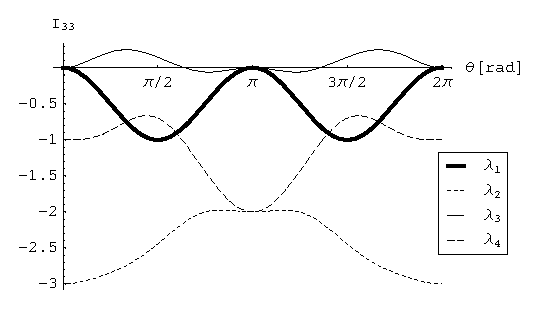
\includegraphics[width=120mm]{2004-qbounds-f11}
\end{itemize}
 }





\section{Uniqueness property and explosion views}
\frame{
\frametitle{Uniqueness property and explosion views [NJP 8, {39} (2005)]}
{\footnotesize
\begin{itemize}
\item<1->
A multipartite state satisfies the {\em uniqueness property} if
knowledge of a property of one quantum entails the certainty
that, if this property
were measured on the other quantum (or quanta) as well, the outcome of the measurement would be
a unique function of the outcome of the measurement performed.

\item<1->
{\em ``Explosion view:''} In analogy to EPR, one might attempt to obtain knowledge of
noncommeasurable observables referring to a single quantum
by measurement of one observable per quantum in a multipartite state satisfying the uniqueness property,
relying on counterfactual inference.

\item<1->
Advantage: No terms present which refer to different detector parameter setups at different times.
In the extreme form, one might hope for an ``simultaneous'' proof of the Kochen-Specker theorem.
Possible measurement of ``contextuality.''

\item<1->
Difficulty: impossibility to find a higher-than-two particle state with the uniqueness property; e.g.,
three-spin 1 particle singlet state:
$$
{1\over \sqrt{6}}(
\vert - + 0\rangle
-
\vert - 0 +\rangle
+
\vert + 0 - \rangle
-
\vert + - 0\rangle
+
\vert 0 - + \rangle
-
\vert 0 + - \rangle
).
$$
\end{itemize}
}
}


%%%%%%%%%%%%%%%%%%%%%%%%%%

\frame{
\centerline{\Large Thank you for your attention!}
 }


\end{document}



 Plot[(1/2)*(((3 - Cos[4*\[Theta]])/2)^(1/2) - 1), {\[Theta], 0, Pi},
   Frame -> True, Filling -> Bottom,
   FrameLabel -> {Style["\[Theta]", FontSize -> 24],
   Style["quantum CH bound", FontSize -> 24]}, AspectRatio -> 1,
 Axes -> True,
 FrameTicks -> {{0, Pi/2,     Pi}, {0, {0.10355, (Sqrt[2] - 1)/4}, {0.207107, (Sqrt[2] - 1)/2}},   None, None}]



Export["h:/mytex/2008-bratislava-ch.pdf", Out[19], "PDF", ImageSize -> 500]








